% !TEX root = ../chap3.tex

\section{Approximation de la partie linéaire}

L'obtention, à l'aide d'un logiciel de calcul formel, de l'exponentielle de la partie linéaire n'est pas toujours envisageable. Il est possible de recourir à une méthode d'approximation pour obtenir une formulation formel de celle-ci qui sera possible d'utiliser pour l'écriture du code de simulation. On s'intéressera dans cette section à la partie linéaire $L$ définie par :
$$
  L = \begin{pmatrix}
    0   & -B_0 & 0          &  0          &  \Omega_{pe}^2 & 0             & 0 \\
    B_0 &  0   & 0          &  0          &  0             & \Omega_{pe}^2 & 0 \\
    0   &  0   & 0          &  0          &  0             & \partial_z    & 0 \\
    0   &  0   & 0          &  0          & -\partial_z    & 0             & 0 \\
   -1   &  0   & 0          & -\partial_z &  0             & 0             & 0 \\
    0   & -1   & \partial_z &  0          &  0             & 0             & 0 \\
    0   &  0   & 0          &  0          &  0             & 0             & -v_z\partial_z \\
  \end{pmatrix}
$$
Cette matrice est de la forme :
$$
  L = \begin{pmatrix}
    A & 0 \\
    0 & -v_z\partial_z
  \end{pmatrix}
$$
matrice diagonale par blocs, dont seul le bloc $A$ pose problème pour calculer formellement l'exponentielle. Ainsi on s'intéressera surtout à la sous-matrice $A$ obtenue après une transformée de Fourier en $z$ du système :
$$
  A = \begin{pmatrix}
    0 & -1 & 0  &  0  &  4  & 0  \\
    1 &  0 & 0  &  0  &  0  & 4  \\
    0 &  0 & 0  &  0  &  0  & ik \\
    0 &  0 & 0  &  0  & -ik & 0  \\
   -1 &  0 & 0  & -ik &  0  & 0  \\
    0 & -1 & ik &  0  &  0  & 0  \\
  \end{pmatrix}
$$
Par abus de notation, nous noterons $A_0$, la matrice $A$ pour $k=0$, ce qui revient à une partie linéaire sans les équations de Maxwell, ceci sera utile lors de la comparaison des résultats entre les méthodes.

\subsection{Troncature de la série de Taylor}
%--------------------------------------------------------------------

On peut définir $e^{tA}$ par la série de Taylor :
$$
  e^{tA} = \sum_{n=0}^\infty \frac{t^nA^n}{n!}.
$$
Une troncature d'ordre suffisamment élevé permet d'obtenir une approximation de l'exponentielle $e^{tA}$ à un ordre plus élevé que la méthode LRK($s$,$n$) où elle sera utilisé garanti que l'erreur de troncature reste inférieur à $n$, l'ordre de la méthode en temps. On définit la troncature de la série de Taylor à l'ordre $p$ par :
$$
  T_p(A) = \sum_{k=0}^p \frac{A^k}{k!}
$$

On sait que les valeurs propres de $A$ sont imaginaires pures, cela signifie que les valeurs propres de $e^{A}$ sont de norme 1.

\begin{figure}
  \begin{subfigure}{.5\textwidth}
    \centering
    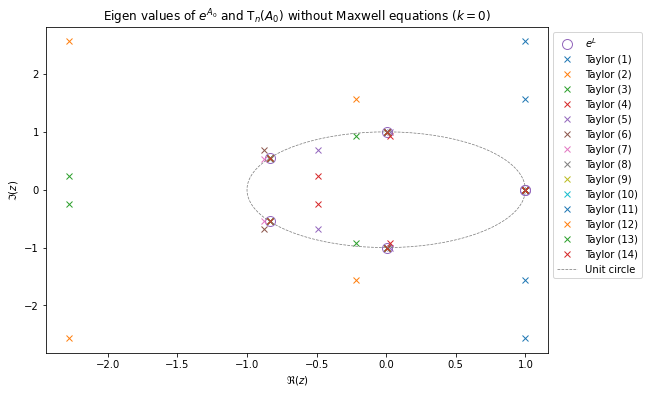
\includegraphics[width=\textwidth]{\localPath/figures/approx_evA0T5.png}
    \caption{Les valeurs propres de $e^{A_0}$ et de $T_5(A_0)$}
  \end{subfigure}
  \begin{subfigure}{.5\textwidth}
    \centering
    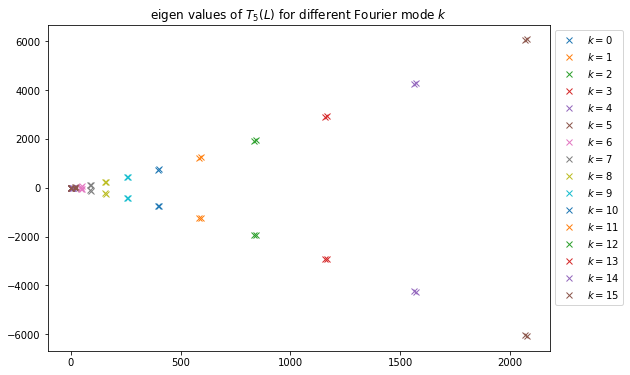
\includegraphics[width=\textwidth]{\localPath/figures/approx_evAkT5.png}
    \caption{Les valeurs propres de $e^{A}$ et de $T_5(A)$ pour différentes valeurs de $k\in[\![0,15]\!]$, par symétrie on obtient aussi celles pour $k<0$}
  \end{subfigure}
  \caption{Valeurs propres de $e^{A}$ et de $T_5(A)$ pour $k=0$ (sans les équations de Maxwell) à gauche, et pour différentes valeurs de $k\in[\![0,15]\!]$ à droite.}
\end{figure}

\Josselin{Je ne sais pas trop quoi dire sur les figures, donc je vais les mettre là un peu en vrac, on pourra discuter de leur intérêt plus tard, mais je pense qu'un petit calcul juste dire que les valeurs propres de $T_p(A)$ ne sont pas de module 1 serait plus intéressant.}

\begin{figure}
  \begin{subfigure}{.5\textwidth}
    \centering
    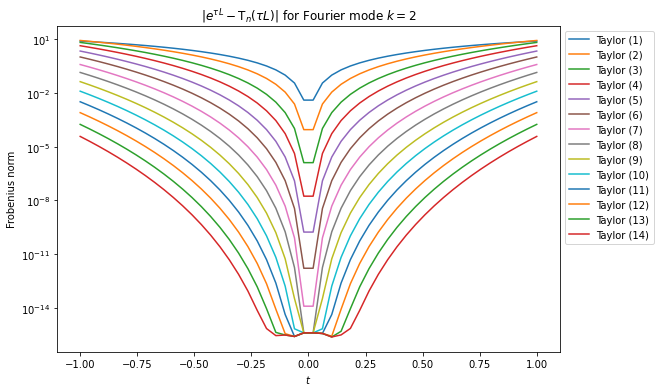
\includegraphics[width=\textwidth]{\localPath/figures/approx_errortA2T.png}
    \caption{L'erreur absolue locale $\|e^{tA}-T_p(tA)\|$ pour le mode de Fourier $k=2$}
  \end{subfigure}
  \begin{subfigure}{.5\textwidth}
    \centering
    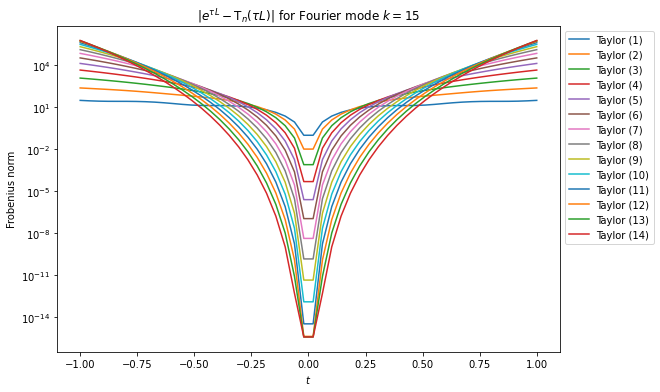
\includegraphics[width=\textwidth]{\localPath/figures/approx_errortA15T.png}
    \caption{L'erreur absolue locale $\|e^{tA}-T_p(tA)\|$ pour le mode de Fourier $k=15$}
  \end{subfigure}
  \caption{Erreur absolue locale $\|e^{tA}-T_p(tA)\|$ pour deux modes de Fourier $k=2$ à gauche et $k=15$ à droite.}
\end{figure}

\begin{figure}
  \centering
  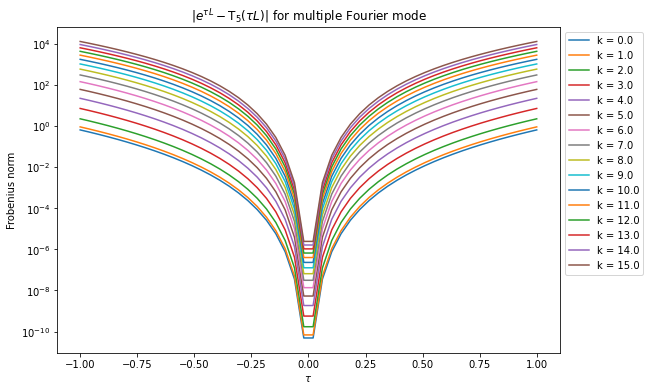
\includegraphics[width=0.75\textwidth]{\localPath/figures/approx_errortAkT5.png}
  \caption{L'erreur absolue locale $\|e^{tA}-T_5(tA)\|$ pour différents mode de Fourier}
\end{figure}

\subsection{Approximant de Padé}
%--------------------------------------------------------------------

Pour approcher une fonction, au lieu d'utiliser un polynôme comme dans le cadre des séries des développement limités, il est possible de construire une fraction rationnelle. L'approximant de Padé de la fonction exponentielle est la meilleure approximation de la fonction exponentielle par une fraction rationnelle et est définie par :
$$
  \begin{aligned}
    h_{p,q}(x) &= \sum_{i=0}^p \frac{\frac{p!}{(p-i)!}}{\frac{(p+q)!}{(p+q-i)!}}\frac{x^i}{i!} \\
    k_{p,q}(x) &= \sum_{j=0}^q (-1)^j \frac{\frac{q!}{(q-j)!}}{\frac{(p+q)!}{(p+q-j)!}} \frac{x^j}{j!}
  \end{aligned}
$$

$$
  p_{p,q}(x) = \frac{h_{p,q}(x)}{k_{p,q}(x)} \approx e^x
$$

Pour utiliser cet approximant de Padé, qui est une fraction rationnelle, avec des matrices il faut utiliser la définition suivante :

$$
  e^M \approx \textrm{P}_{p,q}(M) = h_{p,q}(M)\cdot\left(k_{p,q}(M)\right)^{-1}
$$

On effectue la même étude qu'avec une troncature de la série de Taylor. On regarde donc dans un premier temps sur la figure~\ref{fig:evAP22} les valeurs propres dans le cas $k=0$ et pour différentes valeurs de $k$.

\begin{figure}
  \begin{subfigure}{.5\textwidth}
    \centering
    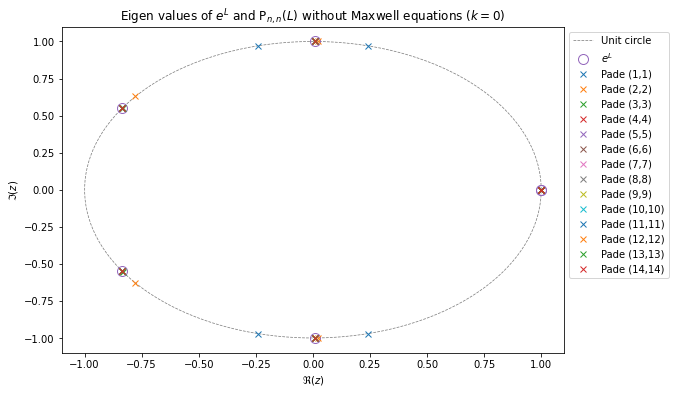
\includegraphics[width=\textwidth]{\localPath/figures/approx_evA0P.png}
    \caption{Les valeurs propres de $e^{A_0}$ et de $P_{n,n}(A_0)$}
  \end{subfigure}
  \begin{subfigure}{.5\textwidth}
    \centering
    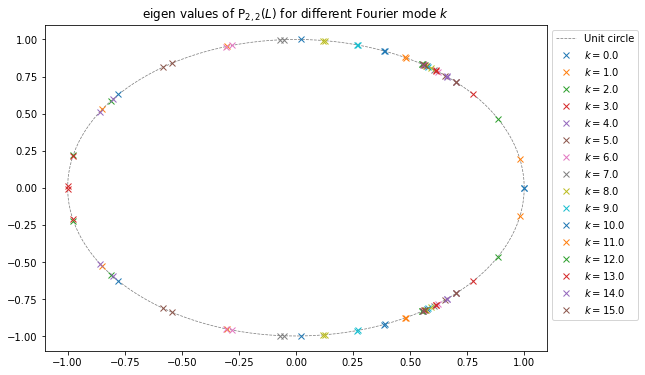
\includegraphics[width=\textwidth]{\localPath/figures/approx_evAkP22.png}
    \caption{Les valeurs propres de $e^{A}$ et de $P_{2,2}(A)$ pour différentes valeurs de $k\in[\![0,15]\!]$, par symétrie on obtient aussi celles pour $k<0$}
  \end{subfigure}
  \caption{Valeurs propres de $e^{A}$ et de $P_{n,n}(A)$ pour $k=0$ (sans les équations de Maxwell) à gauche, et pour différentes valeurs de $k\in[\![0,15]\!]$ à droite.}
  \label{fig:evAP22}
\end{figure}

\begin{figure}
  \begin{subfigure}{.5\textwidth}
    \centering
    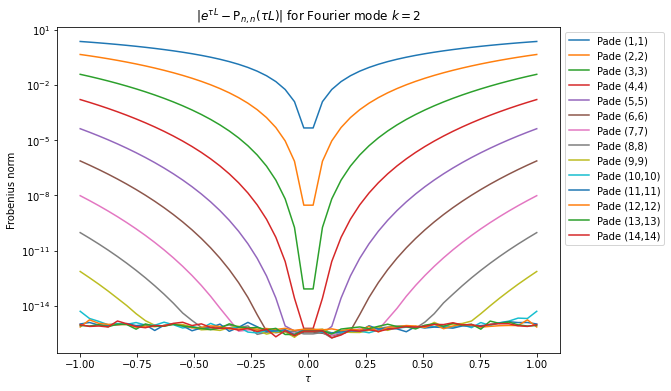
\includegraphics[width=\textwidth]{\localPath/figures/approx_errortA2P.png}
    \caption{L'erreur absolue locale $\|e^{tA}-T_p(tA)\|$ pour le mode de Fourier $k=2$}
  \end{subfigure}
  \begin{subfigure}{.5\textwidth}
    \centering
    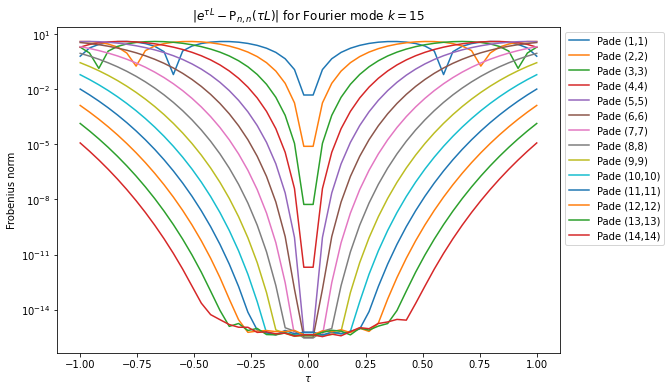
\includegraphics[width=\textwidth]{\localPath/figures/approx_errortA15P.png}
    \caption{L'erreur absolue locale $\|e^{tA}-T_p(tA)\|$ pour le mode de Fourier $k=15$}
  \end{subfigure}
  \caption{Erreur absolue locale $\|e^{tA}-T_p(tA)\|$ pour deux modes de Fourier $k=2$ à gauche et $k=15$ à droite.}
\end{figure}

\begin{figure}
  \centering
  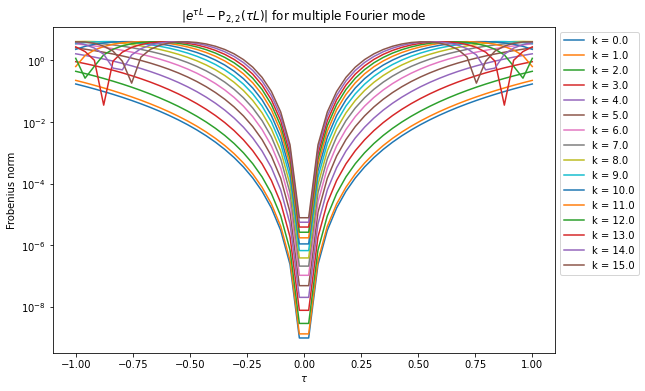
\includegraphics[width=0.75\textwidth]{\localPath/figures/approx_errortAkP22.png}
  \caption{L'erreur absolue locale $\|e^{tA}-T_5(tA)\|$ pour différents mode de Fourier}
\end{figure}


